\documentclass[tikz, border=10 mm]{standalone}
\usepackage[utf8]{vietnam}
\usepackage{tikz}
\usetikzlibrary{calc,decorations.pathmorphing}
\begin{document}
	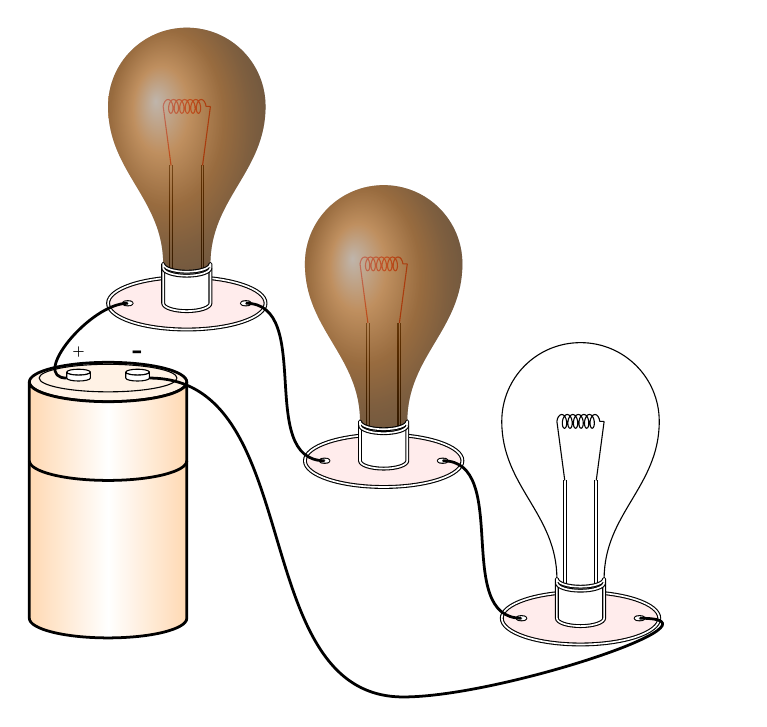
\begin{tikzpicture}[>=stealth,line join=round]
		\def\den[scale=#1](#2){
			\draw[decorate,decoration={coil,segment length=2pt},scale=#1,shift={(#2)}](-0.6,5)--(0.6,5);%Tóc
			\draw [double,scale=#1,shift={(#2)}](-0.4,0.8)--(-0.4,3.5) (0.4,0.8)--(0.4,3.5);
			\draw[scale=#1,shift={(#2)}] (-0.4,3.5)--(-0.6,5) (0.4,3.5)--(0.6,5);
			\draw[scale=#1,shift={(#2)},] (0.6,1) to[out=90,in=-90] (2,5) to [out=90,in =0] (0,7) to[out=180,in=90] (-2,5) to[out=-90,in=90] (-0.6,1) arc (-180:0:{0.6} and {0.2});% bóng
			\draw [scale=#1,shift={(#2)},double, fill=pink!30] (0,0) ellipse ({2} and {2/3});
			\draw[scale=#1,shift={(#2)},fill=white, double] (-0.6,1) arc(-180:0:{0.6} and {0.2}) --++(0,-1) arc (0:-180:{0.6} and {0.2})--cycle;
			\draw[scale=#1,shift={(#2)},double] (-0.6,0.9) arc (-180:0:{0.6} and {0.2});
			\draw [scale=#1,shift={(#2)},double](1.5,0)coordinate(chanhai) ellipse ({0.1} and {0.03});
			\draw [scale=#1,shift={(#2)},double](-1.5,0)coordinate(chanmot) ellipse ({0.1} and {0.03});
		}
		\def\densang[scale=#1](#2){
			\draw[decorate,decoration={coil,segment length=2pt},scale=#1,shift={(#2)},red](-0.6,5)--(0.6,5);%Tóc
			\draw [double,scale=#1,shift={(#2)}](-0.4,0.8)--(-0.4,3.5) (0.4,0.8)--(0.4,3.5);
			\draw[scale=#1,shift={(#2)},red] (-0.4,3.5)--(-0.6,5) (0.4,3.5)--(0.6,5);
			\fill[scale=#1,shift={(#2)},ball color=orange, opacity=0.5] (0.6,1) to[out=90,in=-90] (2,5) to [out=90,in =0] (0,7) to[out=180,in=90] (-2,5) to[out=-90,in=90] (-0.6,1) arc (-180:0:{0.6} and {0.2});% bóng
			\draw [scale=#1,shift={(#2)},double, fill=pink!30] (0,0) ellipse ({2} and {2/3});
			\draw[scale=#1,shift={(#2)},fill=white, double] (-0.6,1) arc(-180:0:{0.6} and {0.2}) --++(0,-1) arc (0:-180:{0.6} and {0.2})--cycle;
			\draw[scale=#1,shift={(#2)},double] (-0.6,0.9) arc (-180:0:{0.6} and {0.2});
			\draw [scale=#1,shift={(#2)},double](1.5,0)coordinate(chanhai) ellipse ({0.1} and {0.03});
			\draw [scale=#1,shift={(#2)},double](-1.5,0)coordinate(chanmot) ellipse ({0.1} and {0.03});
		}
		\def\pin[scale=#1](#2){
			\draw[scale=#1,shift={(#2)},fill=orange!10, line width=1] (0,6) ellipse ({2} and {0.5});
			\fill[scale=#1, shift={(#2)},left color=orange!30, right color=orange!30, middle color=white] (-2,0) arc(-180:0:{2} and {0.5}) --++(0,6) arc(0:-180:{2} and {0.5})--cycle;
			\draw[scale=#1,shift={(#2)}, line width=1](-2,0) arc(-180:0:{2} and {0.5}) --++(0,6) arc(0:-180:{2} and {0.5})--cycle;
			\draw[scale=#1,shift={(#2)}, line width=1](-2,4) arc(-180:0:{2} and {0.5});
			\draw[scale=#1,shift={(#2)}] (0,6.1) ellipse ({1.75} and {0.35});
			\draw[scale=#1,shift={(#2)},fill=white] (0.75,6.25) ellipse ({0.3} and {0.075});
			\draw[scale=#1,shift={(#2)},fill=white] (0.45,6.25) arc(-180:0:{0.3} and {0.075}) --++(0,-0.15)coordinate(am) arc(0:-180:{0.3} and {0.075})--cycle;
			\draw[scale=#1,shift={(#2)},fill=white] (-0.75,6.25) ellipse ({0.3} and {0.075});
			\draw[scale=#1,shift={(#2)},fill=white] (-1.05,6.25) arc(-180:0:{0.3} and {0.075}) --++(0,-0.15) arc(0:-180:{0.3} and {0.075})coordinate(duong)--cycle;
			\draw[scale=#1,shift={(#2)}] (-0.75,6.75) node[scale=#1]{\bf +} (0.75,6.75) node[scale=#1*2]{\bf -} ;
		}
		\densang[scale=0.5](0,8)
		\densang[scale=0.5](5,4)
		\den[scale=0.5](10,0)
		\pin[scale=0.5](-2,0)
		\draw[line width=1] (duong) to [out=180, in=180] ($(chanmot)+(-5,4)$);
		\draw[line width=1] (am) to[out=0, in=180]($(chanhai)+(-3,-1)$) to[out=0,in=0] (chanhai);
		\draw[line width=1] (chanmot) to[out=180,in=0]($(chanhai)+(-2.5,2)$);
		\draw[line width=1] ($(chanmot)+(-2.5,2)$) to[out=180,in=0] ($(chanhai)+(-5,4)$);
	\end{tikzpicture}
\end{document}